\documentclass[a4paper, 14pt]{extarticle}

% Шрифты, кодировки, символьные таблицы, переносы
\usepackage{cmap}
\usepackage[T2A]{fontenc}
\usepackage[utf8x]{inputenc}
\usepackage[english, russian]{babel}

% Пакеты американского математического сообщества
\usepackage{amssymb,amsfonts,amsmath,amsthm}  
% Сокращения
\usepackage{cancel}

\theoremstyle{definition}
\newtheorem{definition}{Определение}

% Красная строка
\usepackage{indentfirst}

% Ссылки в pdf
\usepackage[unicode, colorlinks, urlcolor=magenta, linkcolor=black]{hyperref}

% Таблицы
\usepackage{makecell,multirow} 

% Графика
\usepackage{graphicx}
\usepackage[usenames,dvipsnames]{color} 
\usepackage{float}
% \usepackage{subcaption}

% Геометрия страницы
\usepackage{geometry}
\geometry{left=2cm,right=2cm,top=2.5cm,bottom=2.5cm,bindingoffset=0cm,headheight=18pt}

% Колонтитулы
\usepackage{fancyhdr} 
% применим колонтитул к стилю страницы
\pagestyle{fancy} 
%очистим "шапку" страницы
\fancyhead{} 
%слева сверху на четных и справа на нечетных
\fancyhead[R]{автор(ы)} 
%справа сверху на четных и слева на нечетных
\fancyhead[L]{предмет} 
%очистим "подвал" страницы
\fancyfoot{} 
% номер страницы в нижнем колинтуле в центре
\fancyfoot[C]{\thepage} 

% Межстрочный отступ
\usepackage{setspace}
\linespread{1.15} % капельку увеличенный
\frenchspacing % <<французские>> пробелы

% Нумерация
\renewcommand{\labelenumii}{\theenumii)}
% В заголовках появляется точка, но при ссылке на них ее нет
\usepackage{misccorr}

% Содержание
\usepackage{tocloft}
\usepackage{secdot}
\sectiondot{subsection}

% Физика
\usepackage{physics}

% Новые команды
\newcommand{\Mean}[1]{\langle#1\rangle}
\newcommand{\Defi}{\underset{def}{=}}
\newcommand{\Inte}{\int\limits_{-\infty}^{\infty}} 

\addto\captionsrussian{%
	\renewcommand{\contentsname}{Оглавление}
	\renewcommand{\partname}{Часть}%
}
\def\thepart{\arabic{part}}
\usepackage{tocloft}
\renewcommand{\cftpartleader}{\cftdotfill{\cftdotsep}} % for parts
% \renewcommand{\cftchapleader}{\cftdotfill{\cftdotsep}} % for chapters
\renewcommand{\cftsecleader}{\cftdotfill{\cftdotsep}} % for chapters
% \newlength\mylen
\renewcommand\thepart{\arabic{part}.}
% \renewcommand\cftpartpresnum{Лекция~}
% \renewcommand\cftsecpresnum{Лекция~}
% \setlength{\cftsecnumwidth}{6em}
% \renewcommand{\cftsecpresnum}{Лекция\ }
% \renewcommand{\cftsecaftersnum}{.}
% \renewcommand{\cftsecaftersnumb}{\newline}
\renewcommand{\cftsecdotsep}{\cftdotsep}
\renewcommand{\kappa}{\varkappa}
\renewcommand{\phi}{\varphi}
\renewcommand{\epsilon}{\varepsilon}

% #1: math symbol
% #2: legend
\def\alegend#1#2{\overset{\underset{\scriptstyle\downarrow}{\scriptstyle\text{#2}}}{#1}}
\def\blegend#1#2{\underset{\underset{\scriptstyle\text{#2}}{\scriptstyle\uparrow}}{#1}}
\def\hp{\hat{p}}
\def\hx{\hat{x}}
\def\hH{\hat{H}}

% \usepackage[explicit]{titlesec}
% \titleformat{\section}{\normalfont\Large\bfseries}{}{0em}{Лекция\ \thesection.\ #1}
\usepackage{epigraph}
\usepackage{mathtools}
\mathtoolsset{showonlyrefs=true}

% https://tex.stackexchange.com/questions/8720/overbrace-underbrace-but-with-an-arrow-instead

\usepackage{xparse}% http://ctan.org/pkg/xparse

\NewDocumentCommand{\overarrow}{O{=} O{\uparrow} m}{%
  \overset{\makebox[0pt]{\begin{tabular}{@{}c@{}}$#3$\\[0pt]\ensuremath{#2}\end{tabular}}}{#1}
}
\NewDocumentCommand{\underarrow}{O{=} O{\downarrow} m}{%
  \underset{\makebox[0pt]{\begin{tabular}{@{}c@{}}\ensuremath{#2}\\[0pt]$#3$\end{tabular}}}{#1}
}

\newcommand\undernoteqty[2]{
	%
	\underarrow[
		\qty(\underbrace{#1})
	][\uparrow]{\substack{#2}}
	%
}

\newcommand{\pvec}[1]{\vec{#1}\mkern2mu\vphantom{#1}}
% Нормальный вектор для штрихов

\newcommand\undernote[2]{
	%
	\underarrow[
		#1
	][\uparrow]{\substack{#2}}
	%
}
\DeclareMathOperator{\Div}{div}
\DeclareMathOperator{\Rot}{rot}
\DeclareMathOperator{\Grad}{grad}


\begin{document}
%!TEX root = lectionsA4.tex

% \newpage
\begin{titlepage}
% \thispagestyle{empty}

% \begin{flushleft}
% УДК 532.59(075.8) \\
% ББК 22.251я73\\

% \end{flushleft}
 
% \vskip 20pt
\begin{center}
Министерство науки и высшего образования Российской Федерации
\end{center}
\vskip 20pt
\begin{center}
Федеральное государственное автономное образовательное\\
учреждение высшего образования 
<<Национальный исследовательский Нижегородский государственный университет им. Н.И. Лобачевского>>\\[10pt]
Радиофизический факультет
\end{center}
\vskip 100pt
\begin{center}
	{Автор}
	\vspace{7pt}
\end{center}
\begin{center}
	{\bf \Large НАЗВАНИЕ}
\end{center}
\vskip 20pt
\begin{center}
	\it Учебное пособие
\end{center}
\vskip 20pt
\begin{center}
\fontsize{13pt}{1em}\selectfont
Рекомендовано для студентов
% Оформление и вёрстка: \\ это я
\end{center}

\vfill
\begin{center}
	Нижний Новгород\\
	\currentyear
\end{center}
\vspace{40pt}

\end{titlepage}
\begin{titlepage}
\begin{spacing}{0.92}
\thispagestyle{empty}
% \begin{flushleft}
\noindent\makebox[1.5cm]{УДК} номер номер номер\\ 
% \indent УДК 532, 533.6, 534.2\\ 
% \indent ББК 22.553\\
\noindent\makebox[1.5cm]{ББК}номер\
\noindent\makebox[1.5cm]{}
% \end{flushleft}
\vskip 1em
\begin{center}
	\textit{Рецензенты:}\\
	\textbf{умный человек}~--- д.ф.-м.н., профессор,\\
	\textbf{еще один умный человек}~--- д.ф.-м.н., профессор
\end{center}
\vskip 10pt
\noindent\makebox[1.5cm]{}\textbf{автор авторович}\\
\noindent\makebox[1.5cm]{Г--95}\hspace{1cm}\textbf{название}: учебное пособие /
\begin{adjustwidth}{1.5cm}{0cm}
Автор авторович~--- Нижний Новгород: Изд-во ННГУ им. Н.И. Лобачевского, 2024.~-- много~c.
\end{adjustwidth}
\vskip 10pt
\hspace{2.5cm}ISBN номер
\vskip 10pt
% \fontsize{12pt}{1em}\selectfont

\begin{adjustwidth}{1.5cm}{0cm}
\hspace{1cm}Учебное пособие такое то

% \noindent\hspace{1cm}Публикация данного пособия осуществлена при финансовой поддержке
% Министерства образования и науки Российской Федерации.

\end{adjustwidth}

% Учебное пособие рекомендовано Учёным советом радиофизического факультета
% для студентов ННГУ, обучающихся по направлениям подготовки 03.03.03 и 03.04.03
% ``Радиофизика'' (бакалавриат и магистратура), 02.03.02 ``Фундаментальная информатика и
% информационные технологии'' (бакалавриат), а также специальности 10.05.02
% ``Информационная безопасность телекоммуникационных систем''.

\vskip 1em
\begin{adjustwidth}{1.5cm}{0cm}
\begin{center}
\textit{Ответственный за выпуск:}\\
% заместитель председателя методической комиссии радиофизического факультета ННГУ, 
д.ф.-м.н., профессор умный человек
\end{center}
\vskip 3em
\end{adjustwidth}
% \vfill
\vskip 9em
ISBN номер \hfill УДК номер номер\\
\hphantom{a}\hfill ББК номер
\vskip 2em

\begin{adjustwidth}{6.5cm}{0cm}
\makebox[1cm]{\noindent\tikz[baseline=-0.3em]{\node[left, scale=0.7] (0,0) {\copyright}}}Нижегородский государственный\\
\makebox[1cm]{}университет им. Н.И. Лобачевского, 2024\\
\makebox[1cm]{\noindent\tikz[baseline=-0.3em]{\node[left, scale=0.7] (0,0) {\copyright}}} автор авторович, 2024
\end{adjustwidth}
\end{spacing}
% \end{flushright}

\end{titlepage}

\newpage
\tableofcontents 
\newpage

\part{Электромагнитные волны в линиях передачи}
\begin{figure}[h!]
	\centering
	\includegraphics[width=1\linewidth]{images/grechnev1.png}
	\caption{Изображения солнечного диска 7 августа 2024 года в разных длинах волн}
	\label{grechnev1}
\end{figure}

Обратимся к \cref{grechnev1}. Между изображениями есть определенные сходства, но тем не менее они довольно сильно отличаются друг от друга, и разобраться с запечатленными на снимках в разных спектральных диапазонах процессами обычно довольно проблематично. Часто это осложняется еще и скоротечностью данных процессов.
Для облегчения этой задачи можно использовать совместное использование изображений разных диапазонов, что позволяет более полно восстановить картину происходящего события, установить последовательность явлений и выявить причинно-следственные связи между ними, структуру изучаемого объекта на разных высотах, а также выяснить физические условия в изучаемых объектах и их взаимосвязи.

Совместное использование данных может быть также полезно с точки зрения подтверждения или опровержения догадок, сделанных на основе изучения данных в определенном частотном диапазоне.

\subsection{Одномерные массивы данных (обычно, временные ряды)}
	
В первую очередь, стоит обратить внимание, к какой системе отсчета времени привязан массив данных. Это может быть, например, всемирное время $UT$, определяемое на основе наблюдений за вращением Земли, международное атомное время $TAI$, определяемое через период излучения атома цезия-133, или всемирное координированное время $UTC$, которое учитывает колебания скорости вращения Земли и регулирует эти неточности с помощью дополнительных "<високосных"> секунд, что делает $UTC$ близким к $UT$, но с точностью атомных часов.

\begin{figure}[h!]
	\centering
	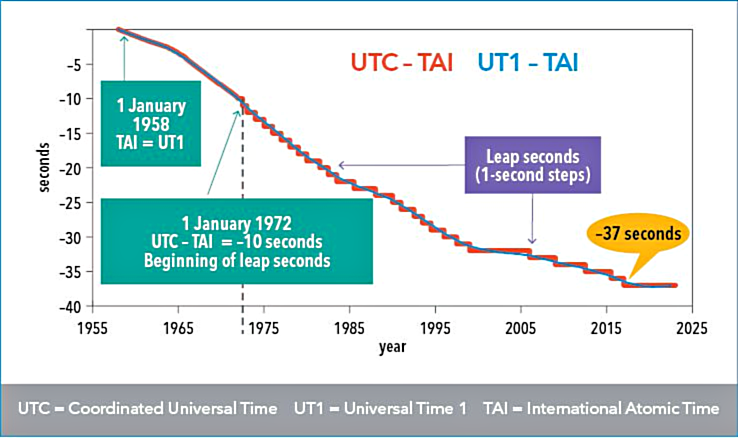
\includegraphics[width=0.55\linewidth]{images/grechnev2.png}
	\caption{Разница между $UT$ и $UTC$}
	\label{grechnev2}
\end{figure}

Разница между $UT$/$UTC$ и $TAI$ составляет, на данный момент, $37$ секунд, что иногда может быть очень существенно. И хоть $TAI$ используется довольно редко, предпочтительнее использовать при анализе одномерных временных рядов зависимость величины не от номера отсчета, а от временной отметки, когда данные были получены. Это поможет избежать ошибок из-за:
\begin{enumerate}
	\item неравномерных отсчетов
	\item записей с пропусками
	\item сбоев записи времени
	\item использования данных с разными шкалами времени
\end{enumerate}
В IDL это можно реализовать путем использования команды:
\begin{python}
	plot, x, y
\end{python}
Или при использовании нескольких графиков с разными шкалами:
\begin{python}
	plot, time1, y1
	oplot, time2, y2
\end{python}
В Python для этого можно использовать:
\begin{python}
	import matplotlib.pyplot as plt
	def format_seconds(x, pos):
	hours = int(x // 3600)
	minutes = int((x % 3600) // 60)
	seconds = int(x % 60)
	return f"{hours:02d}:
	{minutes:02d}:
	{seconds:02d}"
	plt.plot(time, data)
	ax.xaxis.set_major_formatter(
	FuncFormatter(format_seconds))
\end{python}

\begin{figure}[h!]
	\centering
	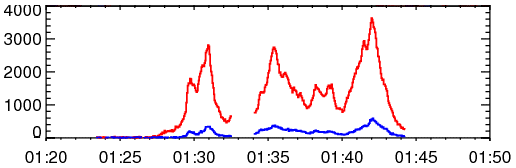
\includegraphics[width=0.65\linewidth]{images/grechnev3.png}
	\caption{Пример правильного отображения данных с пропусками}
	\label{grechnev3}
\end{figure}

Подобный подход позволит создать интерактивную ось времени, при манипуляции с которой (приближении и т. п.) метки останутся верными

Также стоит обратить внимание на валидацию данных и их фильтрацию. К типичным методам можно отнести:
\begin{enumerate}
	\item сглаживание скользящим усреднением: $[1, 4, 100] \Rightarrow 35$
	\item медианное сглаживание: $[1, 4, 100] \Rightarrow 4$\\
	(может быть полезно для оценки стационарного уровня при анализе всплеска излучения)
	\item суммирование отсчетов\\
	(данный подход нужно использовать с осторожностью из-за его фазочувствительности)
	\item Фурье-фильтрация\\
	(разложение исходного сигнала на гармонические составляющие для выделения шумов)
	\item полиномиальная аппроксимация\\
	(повышение порядка полинома повышает точность, но снижает устойчивость)
	\item выделение огибающих и трендов (см. \cref{grechnev4})\\
	(иногда можно заменить аппроксимацией точек минимумов в массиве данных каким-либо способом)
\end{enumerate}

\begin{figure}[h!]
	\centering
	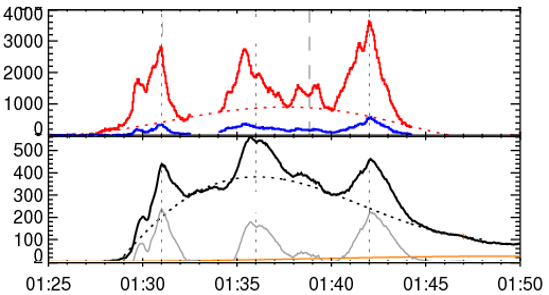
\includegraphics[width=0.65\linewidth]{images/grechnev4.png}
	\caption{Пример использования огибающих}
	\label{grechnev4}
\end{figure}

\subsection{Двумерные массивы данных (обычно, изображения)}

\begin{enumerate}
	\item \textsf{Отображение}
	
	При отображении данных важно правильно подобрать шкалу яркости. Она может быть линейной, степенной, логарифмической, определена какой-то сложной функцией (например, $asinh$), или вообще иметь разные масштабы изменения для разных диапазонов значений (пример -\\ \texttt{matplotlib.colors.TwoSlopeNorm(vcenter, vmin=None, vmax=None)}, что может быть полезно при анализе изображений солнечных вспышек с большим динамическим диапазоном)
	
	\begin{figure}[h!]
		\centering
		\includegraphics[width=0.75\linewidth]{images/grechnev5.png}
		\caption{Пример использования различных шкал яркости. Для случая линейной шкалы выполнено ограничение по порогу}
		\label{grechnev5}
	\end{figure}
	
	\begin{figure}[h!]
		\centering
		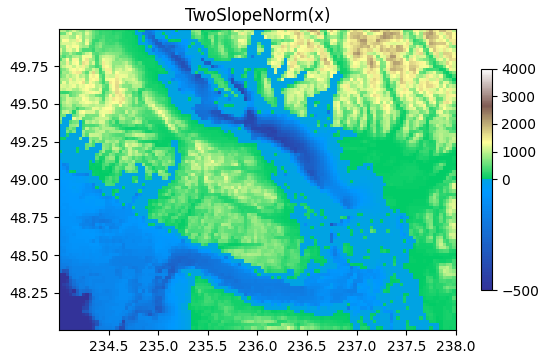
\includegraphics[width=0.7\linewidth]{images/grechnev6.png}
		\caption{Наглядная демонстрация принципа работы нормировки \texttt{TwoSlopeNorm}}
		\label{grechnev6}
	\end{figure}
	
	Также довольно удобным инструментом анализа изображений являются контуры уровня (см. \cref{grechnev7})
	
	\begin{figure}[h!]
		\centering
		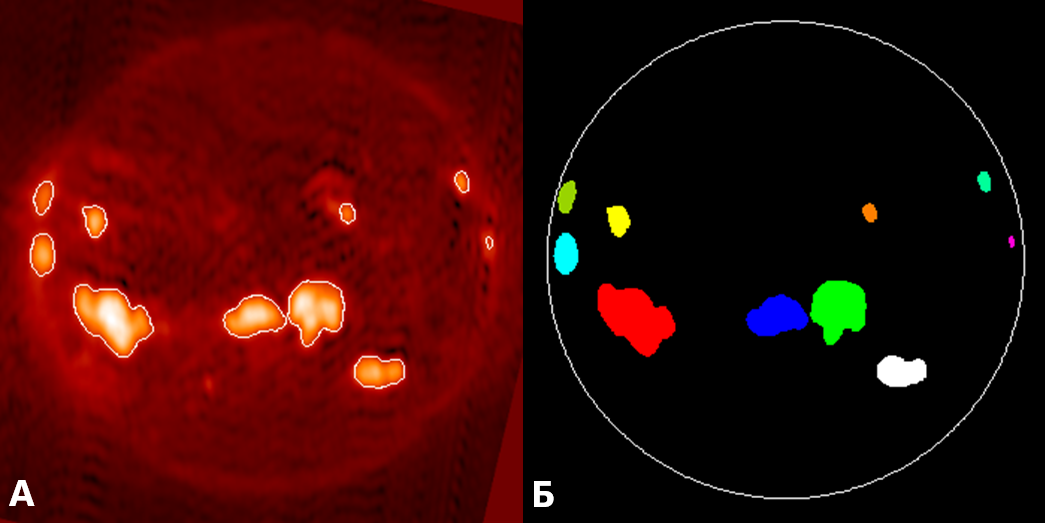
\includegraphics[width=0.7\linewidth]{images/grechnev7.png}
		\caption{А - использование контуров при анализе изображений, Б - "<Раскраска пятен">}
		\label{grechnev7}
	\end{figure}
	
	\item \textsf{Подавление фона и выделение изменений}
	
	Для этой цели широко используется разностные изображения. Их есть два вида: бегущие (последовательные) разности (\textit{Running Difference} - RD) и фиксированные разности (\textit{Fixed Difference} - \textit{FD})
	
	\begin{figure}[h!]
		\centering
		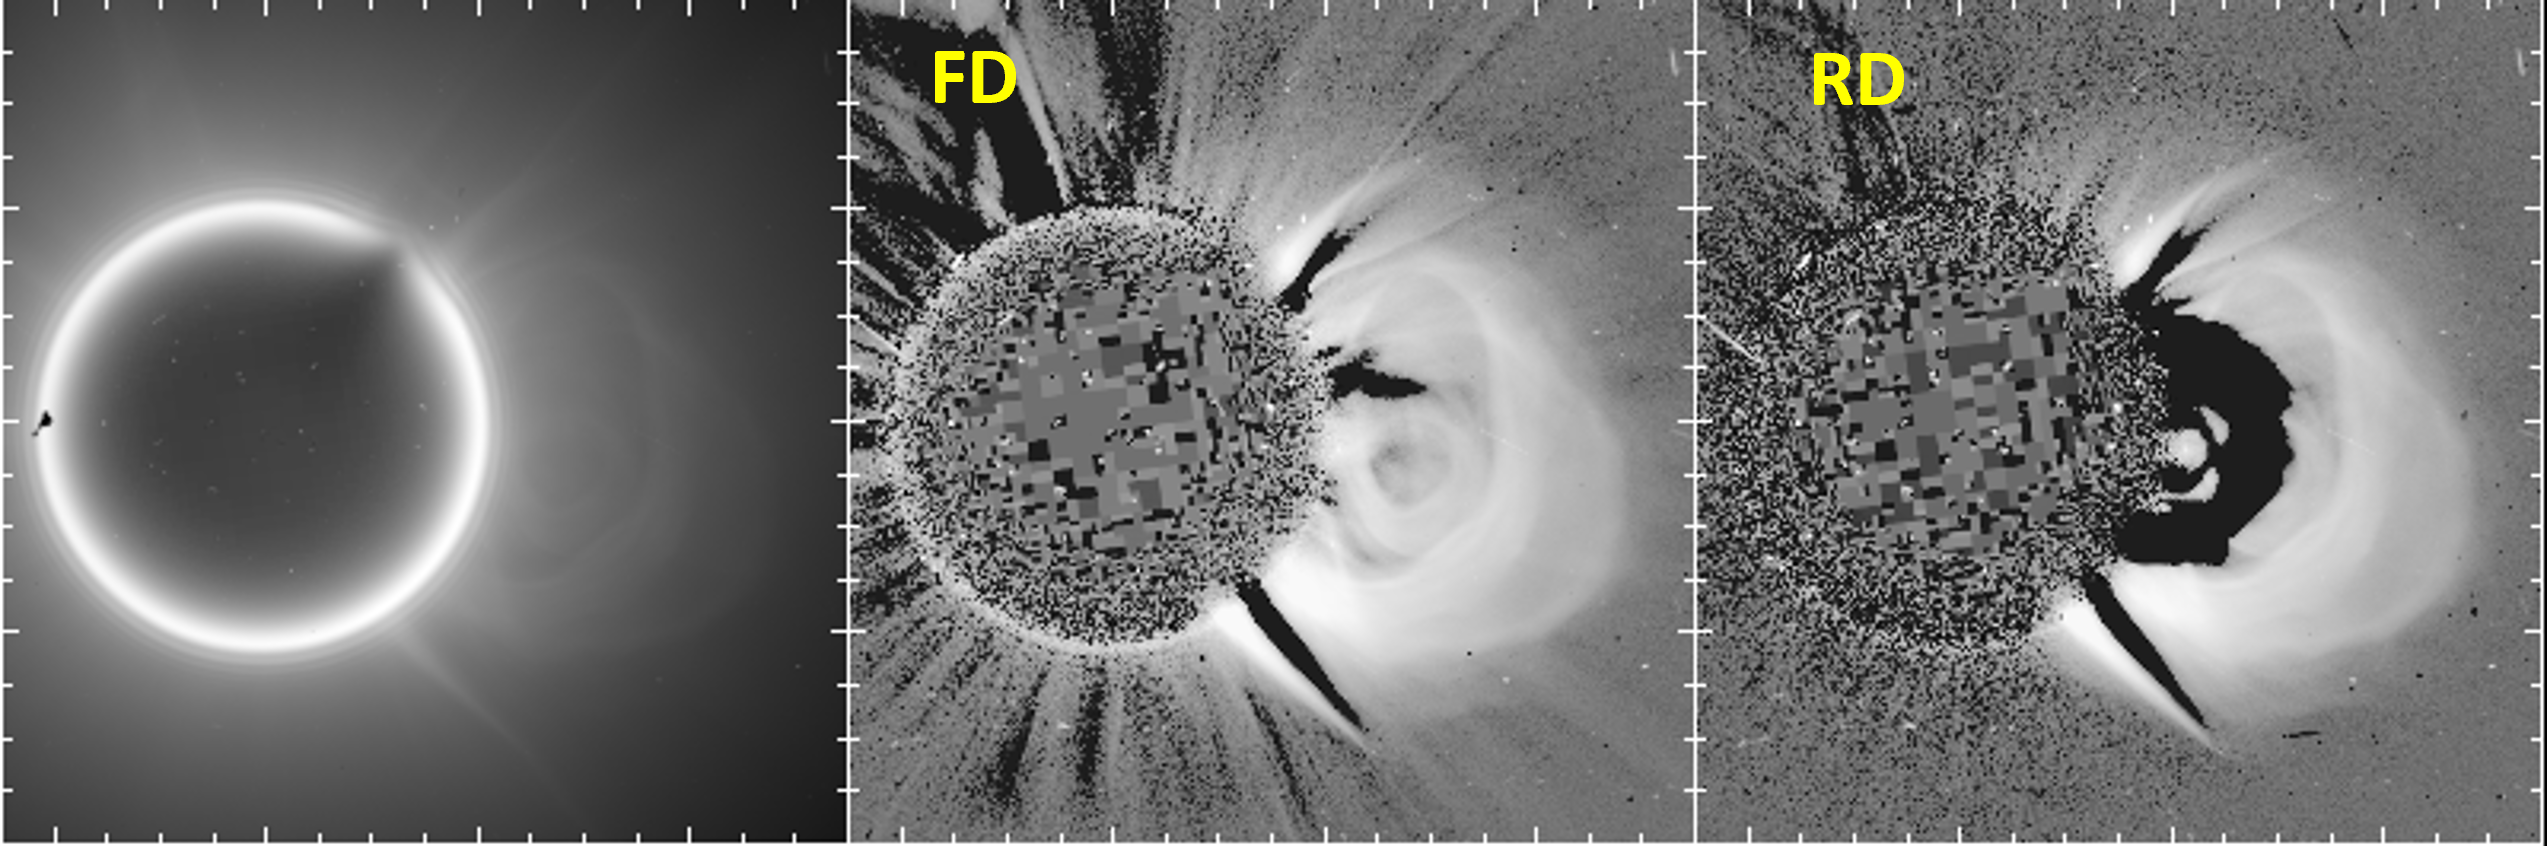
\includegraphics[width=0.7\linewidth]{images/grechnev8.png}
		\caption{Использование разностных изображений. Видно потемнение области }
		\label{grechnev8}
	\end{figure}		
\end{enumerate} 

\section{Волны в линиях передачи с идеально проводящими границами}
\subsection{Дисперсионное уравнение}
Lorem ipsum dolor sit amet, consectetur adipisicing elit, sed do eiusmod
tempor incididunt ut labore et dolore magna aliqua. Ut enim ad minim veniam,
quis nostrud exercitation ullamco laboris nisi ut aliquip ex ea commodo
consequat. Duis aute irure dolor in reprehenderit in voluptate velit esse
cillum dolore eu fugiat nulla pariatur. Excepteur sint occaecat cupidatat non
proident, sunt in culpa qui officia deserunt mollit anim id est laborum. 

\newpage

%!TEX root = ../lections.tex
\subsection{Моды в линиях передачи}
Любая мода в лии передачи характеризуется поперечным волновым числом, а поперечное волновое число определяет продольное.

\begin{figure}[H]
	\centering
	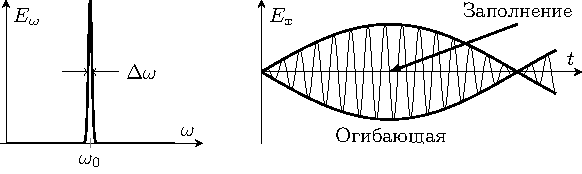
\includegraphics[scale=1.5]{img/lect3_ris8}
	\caption{Квазимонохроматический волновой пакет}
	\label{fig:lect3:8}
\end{figure}

\end{document}